% Web 开发技术现状报告；沿用 ../../项目需求文档/main.tex 的版式。
% 编译：make（XeLaTeX + latexmk）。正文按章节拆分在 chapters/。
\documentclass[12pt,a4paper]{article}
\usepackage[fontset=none]{ctex}
% 正文中西文均采用宋体，强调采用对应粗体；黑体仅用于标题。
\IfFileExists{/System/Library/Fonts/Supplemental/Songti.ttc}{
  \defaultCJKfontfeatures{}
  \setmainfont{Songti.ttc}[Path=/System/Library/Fonts/Supplemental/,FontIndex=6,%
    BoldFont=Songti.ttc,BoldFeatures={FontIndex=1}]
  \setmonofont{Songti.ttc}[Path=/System/Library/Fonts/Supplemental/,FontIndex=6,%
    BoldFont=Songti.ttc,BoldFeatures={FontIndex=1}]
  \setCJKmainfont{Songti.ttc}[Path=/System/Library/Fonts/Supplemental/,FontIndex=6,%
    BoldFont=Songti.ttc,BoldFeatures={FontIndex=1}]
  \setCJKsansfont{STHeiti Light.ttc}[Path=/System/Library/Fonts/,FontIndex=1]
  \setCJKmonofont{Songti.ttc}[Path=/System/Library/Fonts/Supplemental/,FontIndex=6]
  \setCJKfamilyfont{zhsong}{Songti.ttc}[Path=/System/Library/Fonts/Supplemental/,FontIndex=6,%
    BoldFont=Songti.ttc,BoldFeatures={FontIndex=1}]
  \setCJKfamilyfont{zhhei}{STHeiti Light.ttc}[Path=/System/Library/Fonts/,FontIndex=1]
}{
  \defaultCJKfontfeatures{Script=CJK}
  \setmainfont{FandolSong-Regular}[BoldFont=FandolSong-Bold]
  \setmonofont{FandolSong-Regular}[BoldFont=FandolSong-Bold]
  \setCJKmainfont{FandolSong-Regular}[BoldFont=FandolSong-Bold]
  \setCJKsansfont{FandolHei-Regular}[BoldFont=FandolHei-Bold]
  \setCJKmonofont{FandolFang-Regular}
  \setCJKfamilyfont{zhsong}{FandolSong-Regular}[BoldFont=FandolSong-Bold]
  \setCJKfamilyfont{zhhei}{FandolHei-Regular}
}
\providecommand{\songti}{\CJKfamily{zhsong}}
\providecommand{\heiti}{\CJKfamily{zhhei}}
\usepackage[top=2.5cm,bottom=2.5cm,left=3cm,right=2.5cm,headheight=16pt]{geometry}
\usepackage{graphicx,float,booktabs,tabularx,multirow,longtable,array}
\graphicspath{{figures/}}
\usepackage[table]{xcolor}
\definecolor{wmnavy}{HTML}{20354A}
\definecolor{wmaccent}{HTML}{496C86}
\definecolor{wmdivider}{HTML}{D4D8DB}
\usepackage{amsmath,amssymb}
\usepackage{enumitem,caption,needspace,titlesec}
\usepackage{tikz}
\usetikzlibrary{arrows.meta,positioning,shapes.geometric,calc}
\usepackage[unicode=true,colorlinks=true,linkcolor=wmnavy,urlcolor=wmaccent,citecolor=wmnavy,%
  bookmarksnumbered=true]{hyperref}
\usepackage{bookmark}
\usepackage{xurl}
\urlstyle{same}
\newcommand{\sourcecaption}[1]{%
  \par\vspace{1mm}%
  {\footnotesize\color{wmaccent} #1\par}%
}
\hypersetup{pdftitle={Web 开发技术现状报告：从前端入门到展示与内容交互},%
  pdfsubject={WEMOVE-FE-RESEARCH V1.1},pdfauthor={徐熠潘},pdfkeywords={WEMOVE,前端技术,Vue,%
  内容管理,响应式,Web性能}}
\usepackage{fancyhdr}
\pagestyle{fancy}
\fancyhf{}
\fancyhead[L]{\small WEMOVE SPORTS\enspace |\enspace 前端技术报告}
\fancyhead[R]{\small\nouppercase{\leftmark}}
\fancyfoot[C]{\thepage}
\renewcommand{\headrulewidth}{0.4pt}
\renewcommand{\sectionmark}[1]{\markboth{\thesection\enspace #1}{}}
\setcounter{secnumdepth}{3}
\setcounter{tocdepth}{2}
\titleformat{\section}{\Large\heiti}{\thesection}{0.65em}{}
\titleformat{\subsection}{\large\heiti}{\thesubsection}{0.65em}{}
\titleformat{\subsubsection}{\normalsize\heiti}{\thesubsubsection}{0.65em}{}
\titlespacing*{\section}{0pt}{1.2em}{0.8em}
\titlespacing*{\subsection}{0pt}{1em}{0.55em}
\titlespacing*{\subsubsection}{0pt}{0.9em}{0.45em}
\newcommand{\reqheading}[3][4]{%
  \par\Needspace{7\baselineskip}%
  \phantomsection\label{req:#2}%
  \pdfbookmark[#1]{#3}{bookmark:#2}%
  \vspace{0.65em}{\large\heiti\noindent #3\par}%
  \nobreak\vspace{0.35em}\nobreak%
}
\newcommand{\code}[1]{#1}
\newcommand{\smalltable}{%
  \fontsize{11}{16.5}\selectfont%
  \setlength{\tabcolsep}{8pt}%
  \renewcommand{\arraystretch}{1.18}%
  \setlength{\extrarowheight}{4pt}%
  \setlength{\LTpre}{0.65em}%
  \setlength{\LTpost}{0.9em}%
}
\newcolumntype{Y}{>{\raggedright\arraybackslash}X}
\newcommand{\tabledivider}{\arrayrulecolor{wmdivider}\midrule[0.25pt]\arrayrulecolor{black}}
\captionsetup{font=small,labelfont=bf,skip=8pt}
\setlist[enumerate,1]{label=\arabic*.,leftmargin=2.2em,labelsep=0.6em,itemsep=0.35em,parsep=0pt,%
  topsep=0.5em}
\setlist[enumerate,2]{label=\roman*.,leftmargin=2.7em,labelsep=0.6em,itemsep=0.25em,parsep=0pt,%
  topsep=0.35em}
\linespread{1.12}
\setlength{\parskip}{0.35em}
\setlength{\emergencystretch}{2em}
\clubpenalty=10000
\widowpenalty=10000
\displaywidowpenalty=10000
\raggedbottom
\renewcommand{\topfraction}{0.9}
\renewcommand{\bottomfraction}{0.85}
\renewcommand{\textfraction}{0.08}
\renewcommand{\floatpagefraction}{0.85}


\begin{document}
\hypersetup{pageanchor=false}
\begin{titlepage}
\thispagestyle{empty}
\centering
\vspace*{1.6cm}

\includegraphics[width=11cm]{杭电文字 title.png}\par
\vspace{1.45cm}
{\fontsize{34}{46}\selectfont\heiti Web 开发技术现状报告\par}
\vspace{0.8cm}
{\LARGE\heiti 从前端入门到展示与内容交互\par}
\vspace{1.8cm}
\vspace{1.8cm}
\newcommand{\infobox}[1]{\underline{\makebox[7.8cm][c]{\large #1}}}
\renewcommand{\arraystretch}{1.75}
\begin{tabular}{>{\large\heiti}p{2.6cm}l}
课程名称 & \infobox{软件开发实践 2}\\
项目名称 & \infobox{WEMOVE SPORTS 网站重构}\\
报告方向 & \infobox{前端技术、内容与文件管理}\\
姓名 & \infobox{徐熠潘}\\
学号 & \infobox{24051133}\\
日期 & \infobox{2026 年 9 月 7 日}\\
\end{tabular}
\vfill
\end{titlepage}
\pagenumbering{Roman}
\hypersetup{pageanchor=true}
\markboth{摘要}{}
\par\vspace{1.2em}
\noindent\makebox[\textwidth][c]{{\Large\heiti 摘\hspace{0.5em}要}}\par
\nobreak\vspace{0.8em}
本次软件开发实践中，我以前端初学者的身份参与 WEMOVE SPORTS 网站重构，负责站点公共界面、%
文章与品牌内容、常见问题、媒体和资料下载等工作。面对页面布局、交互效果和内容管理任务，我首先调研
HTML、CSS、JavaScript 及其与前端框架、工程工具之间的关系，再结合项目理解 Vue 3、TypeScript、Vue
Router、Pinia、Vite 和浏览器 API 的具体作用。在完成基本页面的基础上，%
我进一步围绕拍立得商品卡片的三维展示、文章与图片的加载、图文内容的编辑三个问题展开技术调查。

报告按照“认识技术—结合任务使用—向相关技术扩展”的顺序，比较 CSS 三维变换、Three.js、WebGL 与 WebGPU
的适用情况，分析客户端渲染、服务端渲染、静态生成、懒加载和响应式图片的优缺点，%
并讨论从原生可编辑区域到结构化编辑器、协同编辑的发展。通过调研，我逐渐认识到，%
前端开发不仅是把页面做得美观，还要协调内容结构、交互状态、设备能力和维护成本。%
通过本项目的开发，我对适度使用三维效果、分清不同资源的加载时机、约束图文结构有了更深入的理解。
\vspace{1.5cm}

\noindent\textbf{关键词：}前端入门；Vue 3；三维展示；内容加载；富文本编辑；Web 开发



\clearpage
\markboth{目录}{}
\begingroup
\setlength{\parskip}{0pt}\linespread{1}\small\selectfont
\tableofcontents
\endgroup
\clearpage
\pagenumbering{arabic}
\section{深入认识前端技术}
\subsection{梳理网页组成}
开始这次任务时，我对前端只有一些粗浅的了解，比如说：知道 three.js 能够帮助网站实现三维效果，但却不知道具体如何使用等等。真正接触项目后，我才第一次从代码层面接触了首页布局、%
菜单展开、文章排版、图片展示和后台编辑等多种多样的前端模块。%
因此，我首先把前端技术按解决的问题分类，然后再决定应该使用什么样的前端工具来完成本项目。

通过调研我了解到：HTML 负责表达内容结构，CSS 负责布局与视觉样式，JavaScript 负责交互与逻辑，%
这是我建立的第一层认识\cite{mdn-basics}。以一张文章卡片为例，标题、图片和链接是内容结构；%
卡片宽度、字距与颜色是样式；点击筛选后重新获取文章是交互。这三者可以类比为展览中的展品目录、%
空间布置与现场工作人员，它们在浏览器中共同作用，共同呈现出一个完整的可交互界面。

浏览器把 HTML 解析成 DOM，即文档对象模型，可以将其理解为一棵由标题、段落、图片等节点组成的树。%
JavaScript 通过 DOM API 读取或修改这些节点；CSS 则影响它们的尺寸、位置和显示方式。%
理解这一点后，我才逐渐明白“把文字放到网页上”和“让网页持续回应用户操作”之间的巨大区别：前者只需呈现内容，%
后者还需要管理事件、数据与页面状态。

\begin{figure}[H]
\centering
\begin{tikzpicture}[font=\fontsize{11}{15}\selectfont,
 box/.style={draw=wmaccent,fill=wmnavy!4,rounded corners=2pt,%
   text width=13.4cm,minimum height=1.15cm,align=center},
 arr/.style={-{Stealth[length=2mm]},draw=wmaccent,line width=0.7pt}]
\node[box] (a) at (0,0) {\textbf{基础：网页有什么，怎样呈现，如何交互}\\%
  HTML 结构 \quad CSS 样式 \quad JavaScript 行为};
\node[box] (b) at (0,-1.6) {\textbf{组织：页面多了以后如何协作与复用}\\%
  Vue 组件 \quad Router 路由 \quad Pinia 共享状态};
\node[box] (c) at (0,-3.2) {\textbf{工程：怎样开发、检查并交付}\\%
  TypeScript 类型 \quad Vite 构建 \quad 测试与浏览器检查};
\node[box,fill=wmaccent!12] (d) at (0,-4.8) {\textbf{任务扩展：如何改善展示和内容操作}\\%
  三维与动效 \quad 内容与图片加载 \quad 图文编辑};
\draw[arr] (a)--(b);%
\draw[arr] (b)--(c);%
\draw[arr] (c)--(d);
\end{tikzpicture}

\caption{我在任务中逐步建立的前端技术地图}%
\label{fig:map}
\end{figure}

\subsection{从基础语言到框架和工程工具}
第二层认识是：框架并不取代 HTML、CSS 和 JavaScript，而是帮助组织它们。%
Vue 的单文件组件将模板、逻辑与样式放在一个组件中，配合响应式状态驱动界面更新\cite{vue-intro}。%
例如，文章列表组件接收数据并显示卡片，公共导航组件统一处理菜单；我不必在每个页面重新写一套相同结构。

我也调研了 React、Svelte 等方案。React 同样以组件组织界面，强调组件、状态和数据流；%
Svelte 则利用编译器转换组件代码\cite{react-ui,svelte-overview}。这些框架的共同点是减少手工维护复杂
DOM 的负担，但语法、状态机制和配套生态不同。%


TypeScript 和 Vite 又属于不同层次。TypeScript 为 JavaScript 增加静态类型检查，%
便于发现字段或参数使用错误；类型标注在编译后会被移除，不能自动验证服务器实际返回的
JSON\cite{ts-basics}。Vite 提供开发服务器、模块更新和生产构建流程，%
解决的是开发与交付效率\cite{vite-why}。

\subsection{基础技术分类}
\begin{table}[!htb]
\centering
\smalltable
\caption{前端技术分别解决什么问题}
\begin{tabularx}{\linewidth}{>{\raggedright\arraybackslash}p{2.4cm}YY}
\toprule
层次 & 代表技术 & 我在项目中对应的理解\\
\midrule
内容与样式 & HTML、CSS、Flexbox、Grid & 组织文章、排列导航和卡片，适应不同页面宽度\\
\tabledivider
行为与平台能力 &
    JavaScript、DOM、Fetch、事件、动画 API &
    读取数据、响应点击、控制加载状态和动态效果\\
\tabledivider
组件与状态组织 & Vue、Router、Pinia & 复用页面结构，切换地址，共享必要的会话状态\\
\tabledivider
工程与质量 & TypeScript、Vite、Vitest & 提前发现错误、构建资源、检查关键交互逻辑\\
\tabledivider
专题展示与内容生产 & Three.js、图片加载、富文本编辑器 & 为具体体验补充能力，而非每个页面全部引入\\
\bottomrule
\end{tabularx}
\end{table}

这次分类还帮助我区分了两个容易混淆的“响应式”：Vue 的响应式是数据变化后界面跟着更新，CSS
的响应式设计是布局随可用空间变化。前者主要处理数据与视图的关系，后者处理内容与屏幕的关系。%


\section{在项目中使用前端技术}
\subsection{学习内容对应具体任务}
我在本次实践中的具体方向是站点、内容与文件，包括公共导航、首页与品牌展示、玩法文章、FAQ、下载中心，%
以及内容和媒体管理页面\cite{local-team}。这些页面既服务于阅读内容的访客，也服务于维护内容的管理员。%


在公共布局中，我接触到组件复用、路由和响应式样式；在文章页面中，我需要理解接口读取、%
异步状态和图文排版；在管理界面中，我又进一步接触表单、文件、选区和版本冲突。%
表\ref{tab:used}整理了当前工程实际使用的技术及其位置。

\begin{table}[!htb]
\centering
\smalltable
\caption{本项目实际使用的前端技术}%
\label{tab:used}
\begin{tabularx}{\linewidth}{>{\raggedright\arraybackslash}p{2.75cm}YY}
\toprule
技术 & 具体用途 & 能力边界\\
\midrule
Vue 3 与组合式 API & 公共导航、文章列表、编辑器和状态组件 & 组织界面与逻辑；不能代替后端数据校验\\
\tabledivider
TypeScript & 内容、媒体、文件等接口类型；组件参数 & 提供编译期约束；外部响应仍需运行时判断\\
\tabledivider
Vue Router 与 Pinia & 页面导航、路由懒加载、会话共享 & 管理端入口判断不等于服务端授权\\
\tabledivider
Element Plus & 管理页面中的现成对话框等界面组件 & 提供组件库能力，与 Vue 的组件机制不是同一层\\
\tabledivider
CSS Grid / Flexbox & 图文并列、卡片网格、窄屏单列 & 布局正确仍需在具体视口下检查\\
\tabledivider
Fetch 与异步逻辑 & 读取文章、筛选资料、提交内容 & 请求可能乱序、失败或结果暂时不确定\\
\tabledivider
Three.js CSS3DRenderer & 拍立得商品卡片的倾斜与回弹 & 变换的是 DOM 元素，不是实体商品三维模型\\
\tabledivider
浏览器动画与观察 API & 页面入场、可见性判断、逐帧运动 & 特性或设备条件不足时保留静态内容\\
\tabledivider
原生编辑能力与自制区块 & 文字格式、左右图文、图注和预览 & 支持受控内容结构，未实现多人实时协作\\
\bottomrule
\end{tabularx}
\end{table}

\subsection{三个让我继续深入调研的问题}

第一个问题来自商品展示：一张图片怎样看起来像可以轻轻拿起的相纸？%
最开始我把这种立体感理解为“制作一个三维模型”，但代码中的 CSS3DRenderer
变换的其实是包含图片和文字的 DOM。这个差别使我继续查阅 CSS 三维、WebGL 和 WebGPU，%
理解不同层次的“网页三维”。

第二个问题来自内容页面：打开文章时，页面代码、文章数据和图片为什么不是同时出现？%
项目的路由使用动态 import，详情页又通过接口读取文章，正文图片还设置了懒加载。%
这说明“加载页面”至少包含加载代码、读取数据、获取图片和完成绘制几个过程。%


第三个问题来自后台编辑：为什么看起来只是一块可以输入文字的区域，却要处理图注、粘贴、%
段落结构和重复保存？当前编辑器既要让管理员方便操作，又要保证前台能稳定展示。%
因此，我从 contenteditable 延伸到结构化编辑器，进一步了解内容模型、事务和协作机制。%
这三个问题构成后续调研的主线。

\subsection{从页面效果理解组件和状态}
在 Vue 中，我逐渐形成“界面是当前状态的结果”的理解，可简写为
\[
\text{界面}=F(\text{数据},\text{交互状态}).
\]
例如，同一个文章区域可以显示加载提示、成功内容、空结果或错误提示。组件化让这些状态拥有统一表现，%
但并不会自动替我决定失败后保留哪些输入、是否允许重试。项目中的 ContentState、ContentBody 和
ContentEditor 分别承担状态展示、正文渲染与编辑职责；把它们区分开后，%
排查问题会比让一个页面处理所有细节清楚得多。

\section{从卡片动效到三维展示}
\subsection{我在项目中接触的三维效果}
WEMOVE 的商品展示使用拍立得风格卡片。鼠标移动时，卡片轻微倾斜，离开后平稳回到原位。%
它给人的感觉接近拿起一张相纸，但卡片里的商品仍是二维图片。当前 PolaroidMotion 使用 Three.js 的
CSS3DObject 和 CSS3DRenderer，将已有 DOM 放入场景并进行位置、%
旋转和缩放变换\cite{local-code,three-css3d}。

项目先把鼠标在卡片中的位置归一化。以水平方向为例，若鼠标位置为 $x$，卡片左边界为 $x_0$、宽度为
$w$，则
\[
u=\operatorname{clamp}\!\left(2\frac{x-x_0}{w}-1,-1,1\right).
\]
当鼠标从左到右移动时，$u$ 从约 $-1$ 变化到 $1$，再映射为小角度旋转。%
组件使用平滑跟随而不是立即跳到目标角度，因而产生柔和的回弹。这里的数学作用很具体：%
把不同卡片尺寸下的鼠标位置转换成可比较的交互输入。

动画由 requestAnimationFrame 驱动，并根据实际帧间隔调整变化。稳定后停止继续申请帧，%
可以避免静止卡片仍持续计算。若以 60 帧每秒为例，每帧总时间约为 $1000/60\approx16.7$ 毫秒，脚本、%
布局和绘制需要共享这段时间。项目还响应减少动画偏好，在失焦或页面可见性变化时重置运动。%
对这种装饰性效果，静态展示本身就应该完整。

\subsection{CSS 三维与 WebGL：看起来相似，工作对象不同}
CSS transform 和 perspective 能让网页元素产生透视旋转；CSS3DRenderer 则帮助用相机、%
场景和对象的方式管理此类 DOM 变换\cite{three-css3d}。优势是可以保留现有文字、图片与链接，%
较容易融入页面；限制是它并不提供网格材质、真实灯光与阴影系统。官方还注明该渲染器只支持 100\%
浏览器和显示缩放，因此放大浏览时的展示需要额外检查，装饰性效果应有静态退路。%
对只有几张卡片的效果，直接使用 CSS 变换也可能足够，引入库的收益应与依赖成本一起考虑。

WebGL 面向 GPU 加速图形，在画布上绘制几何体、纹理和着色结果。Three.js 在其上提供场景、相机、%
几何体、材质等较高层抽象\cite{three-fundamentals}。可以把场景理解为摄影棚，相机决定观察角度，%
几何体决定物体形状，材质与光照共同影响外观，渲染器负责形成图像。%
图\ref{fig:three-official}展示了这些对象之间的关系。

\begin{figure}[H]
\centering
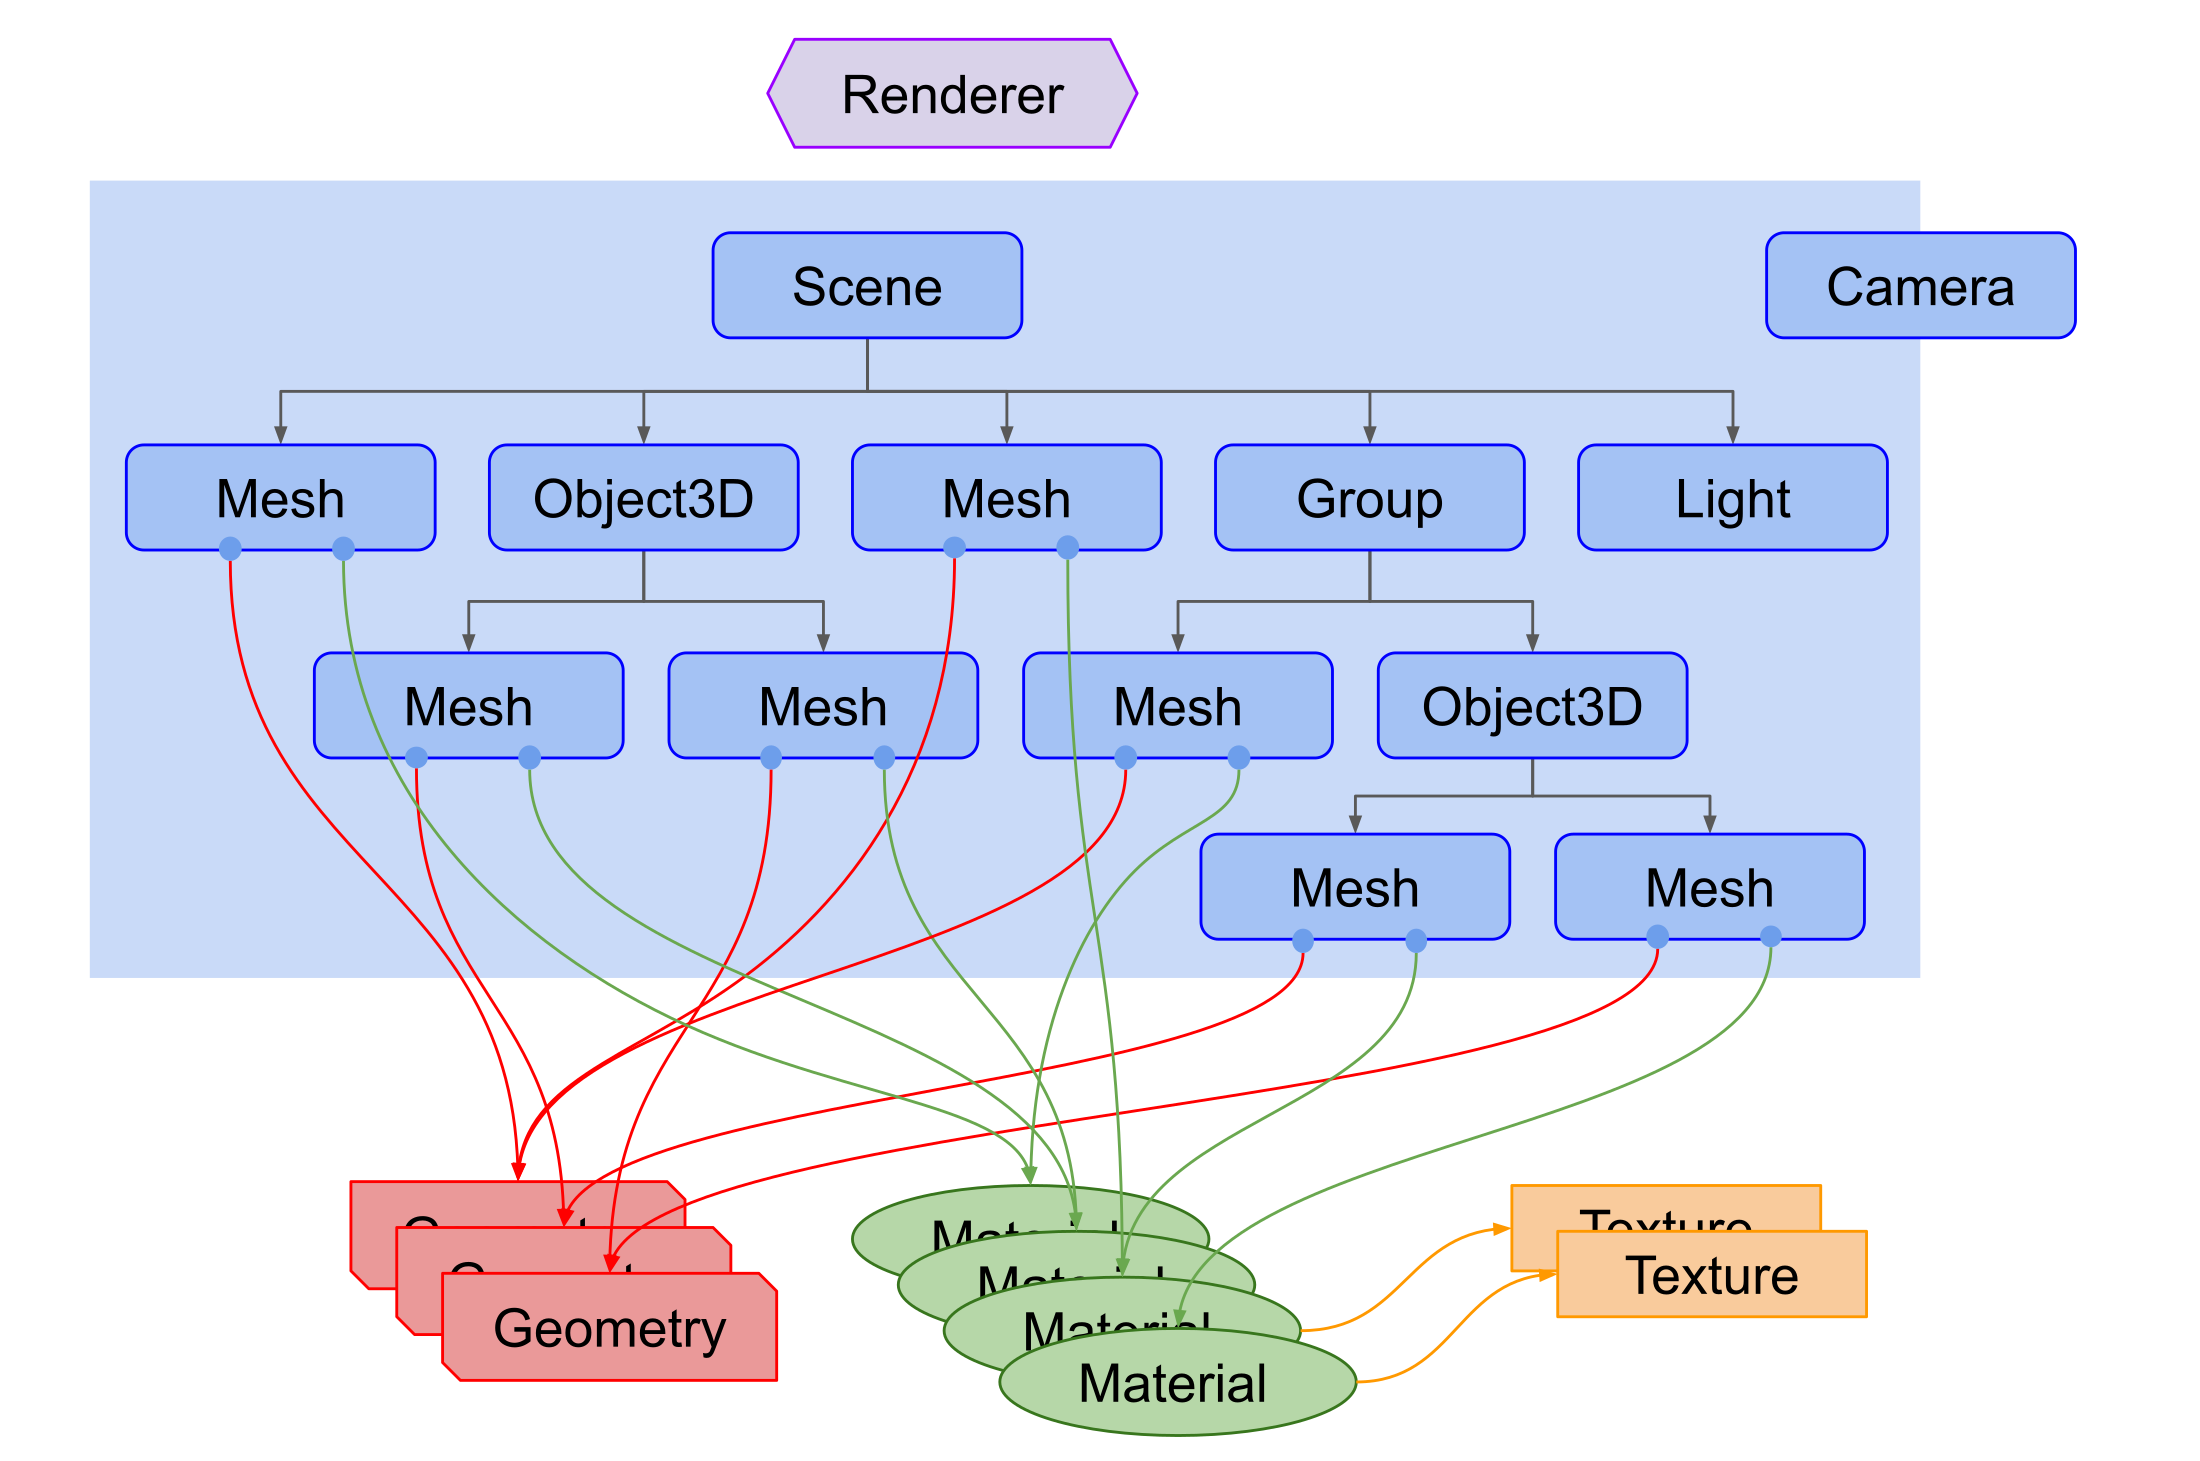
\includegraphics[width=0.91\linewidth]{online/three-structure.png}
\caption{Three.js 官方手册中的网格场景与渲染对象关系}%
\label{fig:three-official}
\end{figure}

透视相机还有“看得见的范围”。视锥由视角、宽高比和近远裁剪平面共同限定，图\ref{fig:frustum}中的
near、far 分别表示近端与远端边界。在简化的针孔模型中，可将正向距离记为 $z$，水平投影写成
$x'=fx/z$：同一尺寸的物体越远，投影越小。

\begin{figure}[H]
\centering
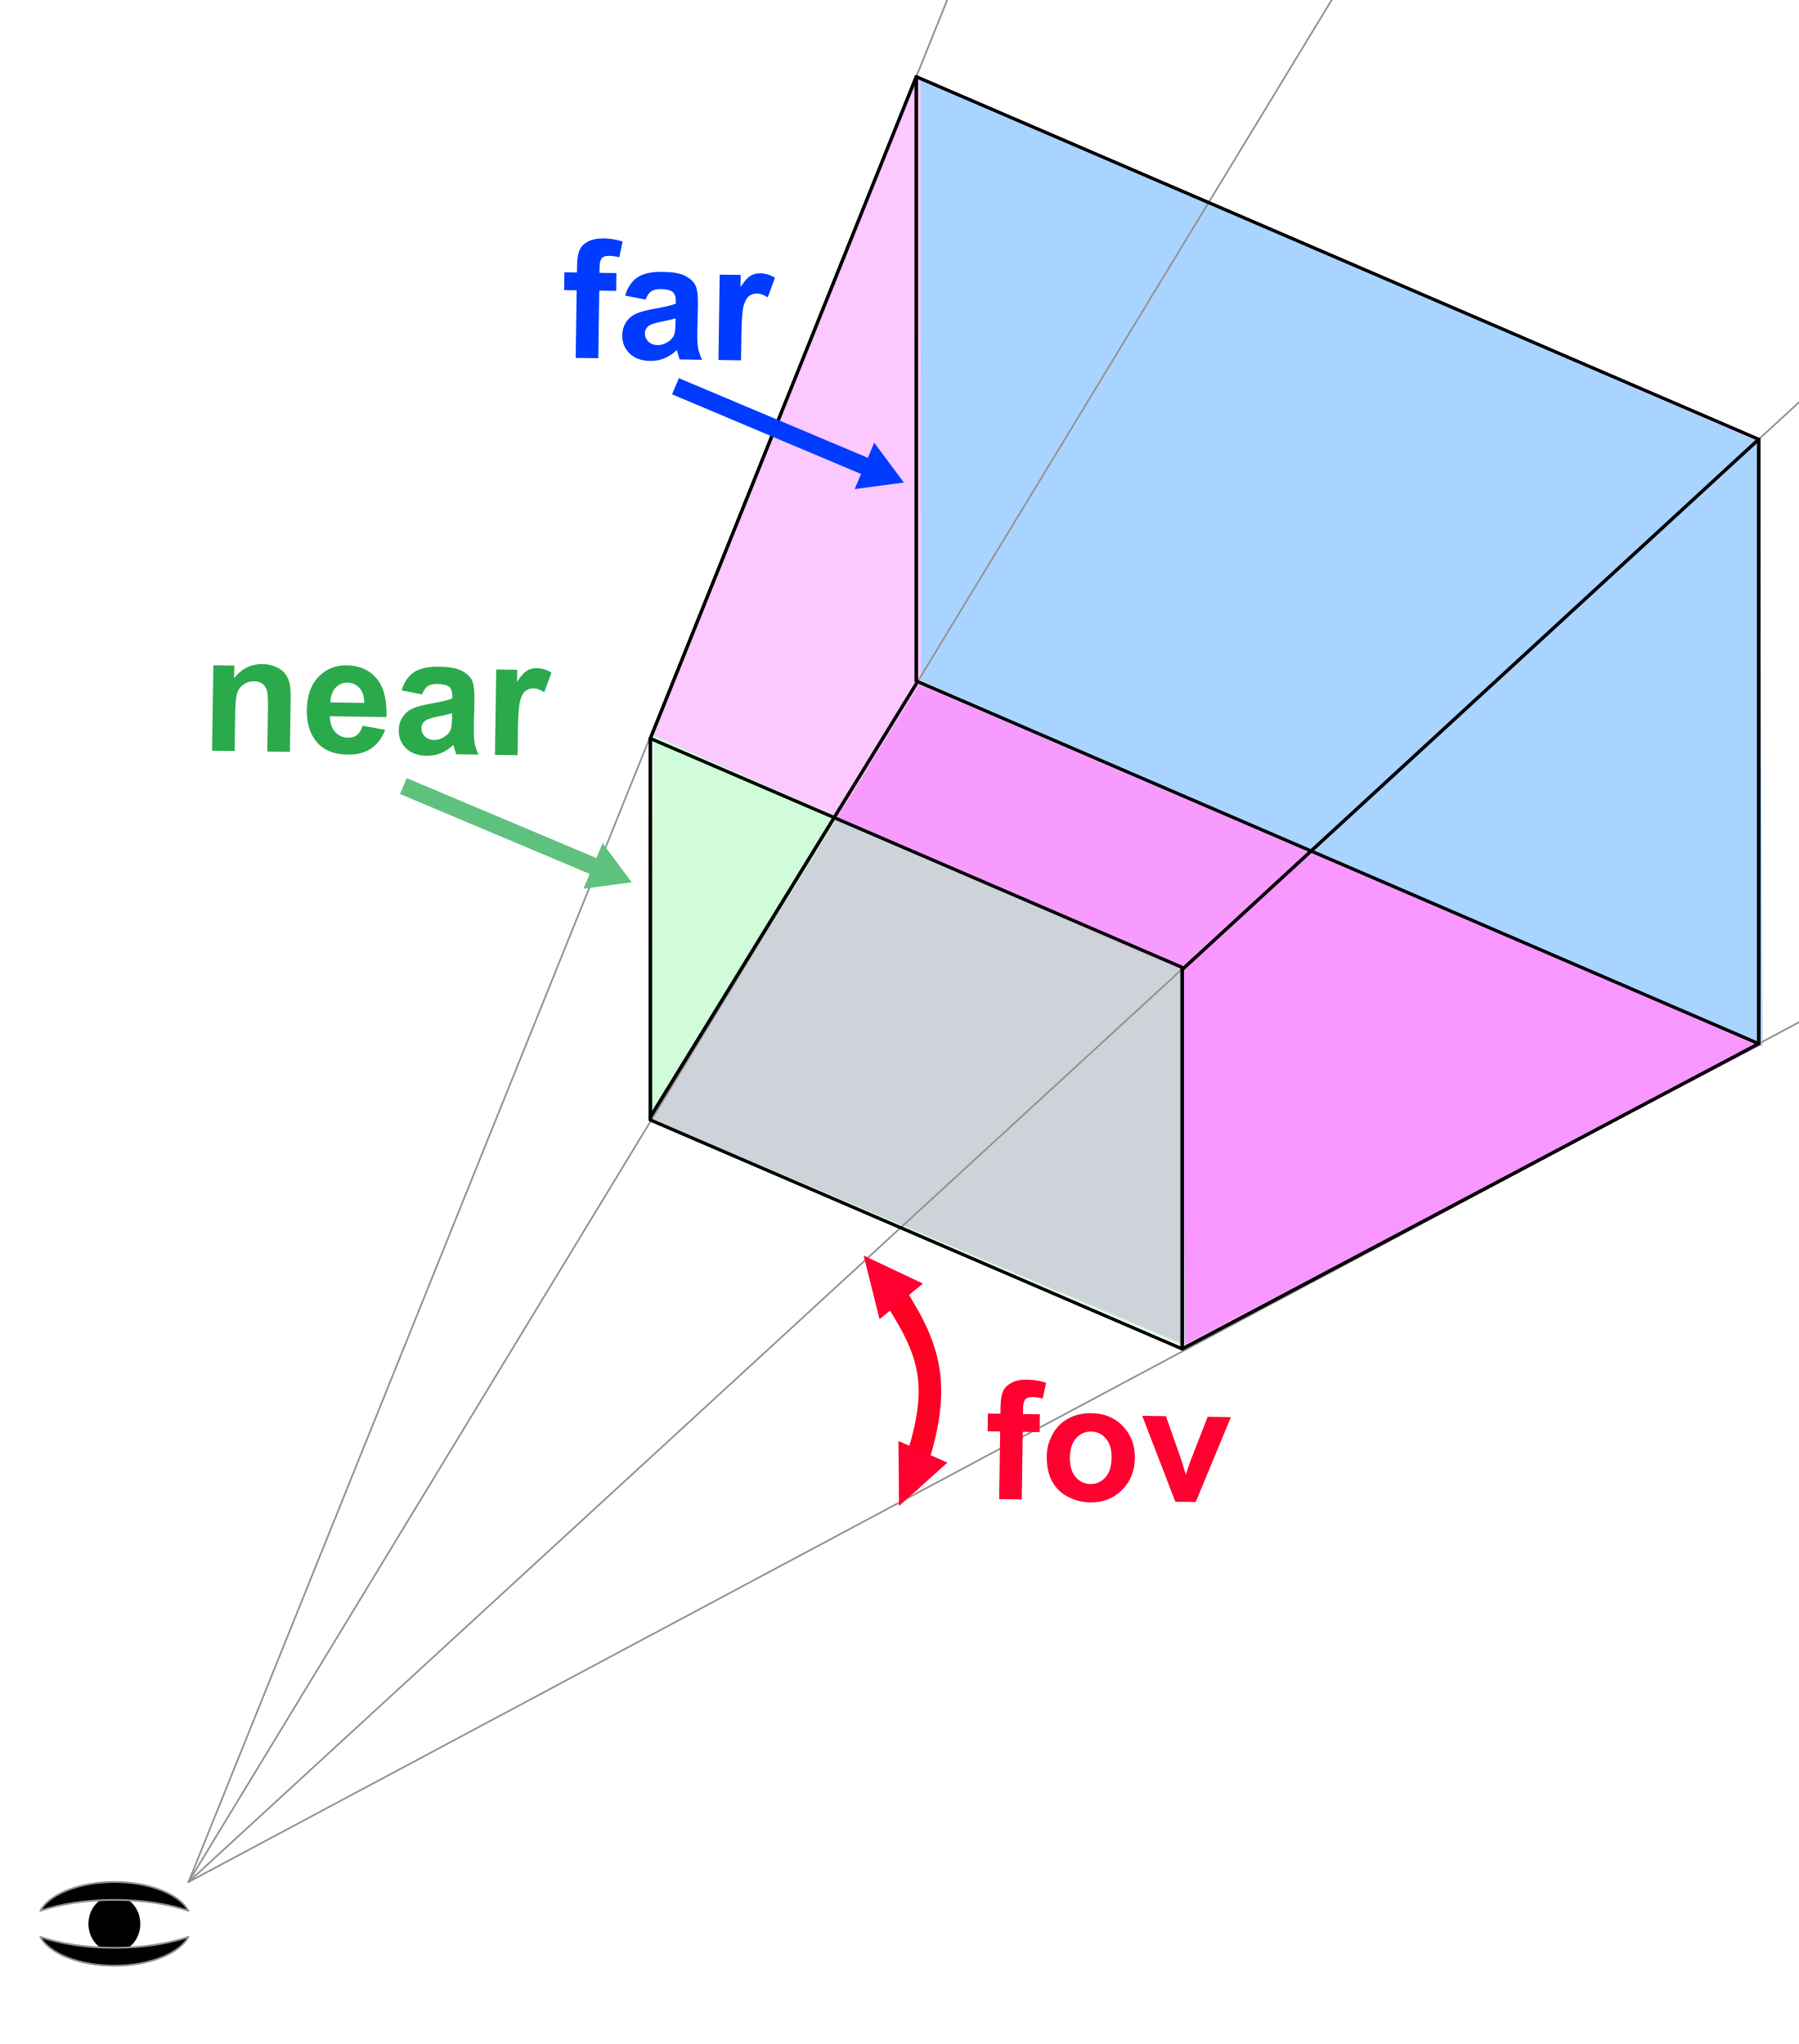
\includegraphics[width=0.73\linewidth]{online/three-frustum.png}
\caption{Three.js 官方透视相机视锥示意}%
\label{fig:frustum}
\end{figure}

如果任务变成“让顾客旋转查看商品背面”，就需要真实三维资产及其加载、材质和交互方案，%
单张图片倾斜无法补出背面的形状。WebGL 适合三维产品预览、可视化场景和浏览器游戏，%
但开发者还需管理模型体积、纹理分辨率、加载时间、设备性能及画布之外的文字说明。%
技术升级带来的不仅是视觉自由度，也包括资产制作和维护工作。

\subsection{WebGPU 与更高层的三维展示工具}
进一步调研后，我发现网页图形正在向更现代的 GPU 接口发展。WebGPU 既提供图形渲染能力，%
也提供计算能力；其资源与管线组织方式和 WebGL 不同\cite{mdn-webgpu}。Three.js 的 WebGPURenderer
提供了较高层入口，并在其文档所述条件下提供 WebGL 2 回退路径\cite{three-webgpu}。%
官方手册当前仍将这一渲染器描述为实验状态。回退是 Three.js 渲染器提供的能力，原生 WebGPU
不会自动转换成 WebGL；节点材质与 TSL（Three.js 着色语言）等组织方式，也使基于 ShaderMaterial
的旧自定义着色器需要迁移。

另一条路线是提高抽象层级。例如 model-viewer 用 Web 组件提供模型展示和相机交互，适合围绕 glTF
等模型资产进行产品预览\cite{model-viewer}。它减少了从零搭建场景的工作，%
但也把能力限制在组件提供的接口范围内。由此我理解到，选择底层 API、通用三维引擎还是成品展示组件，%
本质上是在控制自由度与实现成本之间做取舍。

\begin{table}[!htb]
\centering
\smalltable
\caption{三维展示路线的优缺点与适用场景}
\begin{tabularx}{\linewidth}{>{\raggedright\arraybackslash}p{2.6cm}YY}
\toprule
路线 & 优点与适合任务 & 主要代价或限制\\
\midrule
CSS / CSS3DRenderer &
    保留 DOM 内容，适合卡片、相册和空间化界面 &
    不是实体模型渲染，缺少网格材质能力，并有缩放支持限制\\
\tabledivider
Three.js + WebGL & 适合自定义模型、材质、场景和交互 & 需要三维资产、性能优化和较多图形学知识\\
\tabledivider
Three.js + WebGPU &
    面向新图形与计算能力，保留较高层场景组织 &
    兼容性、回退及特性差异要按目标环境核查\\
\tabledivider
model-viewer & 较快建立模型浏览与交互入口 & 定制深度受组件接口限制，模型优化仍需负责\\
\bottomrule
\end{tabularx}
\sourcecaption{根据官方资料归纳\cite{three-css3d,three-fundamentals,three-webgpu,model-viewer}。%
    未对本项目进行跨方案跑分。}
\end{table}

对当前任务，我更认同“让效果服务于展示目标”：拍立得倾斜要突出卡片的轻盈和互动感，%
不需要为此加载复杂商品网格；只有任务确实要求观察实体空间结构时，才值得引入完整模型链路。%
三维效果的发展方向可以很先进，而一个小项目的合理选择仍可以很克制。

\section{从打开文章到内容加载}
\subsection{一个页面其实有几种不同的加载}
在文章页任务中，我开始区分代码、数据与媒体资源。代码决定页面怎么运行，接口数据提供文章标题和正文，%
图片文件提供实际画面。项目的路由动态 import 解决页面代码什么时候下载的问题，%
接口请求解决内容什么时候到达的问题，图片懒加载解决哪些图片暂时不需要读取的问题。%
它们都叫“按需加载”，却作用在不同对象上。

Vue Router 支持以动态导入定义路由组件，浏览器访问对应路由时再获取相关代码\cite{router-lazy}。%
这适合把后台编辑器等非首屏功能从普通访客的初始路径中分离出来。%
代价是第一次切换到该页面时可能增加一次等待，所以仍需要清楚的加载反馈，%
并检查共享依赖是否被其他入口提前引入。写了动态 import 并不能保证所有资源都已实现最优拆分。

数据加载则需要考虑请求之间的关系。当前文章详情先读取正文，关联商品读取失败时仍保留文章；%
列表使用请求序号，避免较早搜索的慢响应覆盖新的筛选结果\cite{local-code}。%
我把它理解为“只接纳最新一次问题的答案”，而不是“谁最后送到就显示谁”。取消请求可以减少无效工作，%
但提交结果前仍要检查它是否属于当前页面意图。

\subsection{正文在浏览器生成，还是提前生成}
客户端渲染（CSR）主要在浏览器执行 JavaScript 后形成业务正文；服务端渲染（SSR）在处理请求时生成
HTML；静态生成（SSG）在构建时提前生成 HTML\cite{vue-ssr}。水合则是客户端把组件状态和事件连接到已存在
HTML 的过程。对初学者而言，最容易抓住的区别是：用户拿到初始 HTML 时，%
里面是否已经有可阅读的文章内容。

\begin{figure}[H]
\centering
\begin{tikzpicture}[
  font=\fontsize{10.5}{14}\selectfont,
  stage/.style={draw=wmnavy!65,fill=white,rounded corners=2pt,
    text width=3.0cm,minimum height=1.35cm,align=center,
    inner sep=4pt,line width=0.6pt},
  link/.style={-{Stealth[length=2mm]},draw=wmaccent,line width=0.7pt}
]
\node[anchor=west,font=\fontsize{11}{14}\selectfont\bfseries,text=wmnavy]
  at (0,1.05) {CSR：客户端渲染};
\node[stage] (c1) at (1.65,0) {浏览器\\请求页面};
\node[stage,fill=wmnavy!5] (c2) at (5.4,0) {返回 HTML 壳\\通常缺少主要正文};
\node[stage] (c3) at (9.15,0) {浏览器执行 JS\\获取数据并渲染};
\node[stage,fill=wmnavy!9] (c4) at (12.9,0) {主要正文出现\\建立页面交互};
\draw[link] (c1) -- (c2);
\draw[link] (c2) -- (c3);
\draw[link] (c3) -- (c4);
\node[anchor=west,font=\fontsize{11}{14}\selectfont\bfseries,text=wmnavy]
  at (0,-1.35) {SSR：服务端渲染};
\node[stage] (r1) at (1.65,-2.4) {浏览器\\请求页面};
\node[stage,fill=wmnavy!9] (r2) at (5.4,-2.4) {服务端生成页面\\HTML 已含正文};
\node[stage,fill=wmnavy!9] (r3) at (9.15,-2.4) {浏览器显示正文\\此时可未执行 JS};
\node[stage] (r4) at (12.9,-2.4) {执行 JS 并水合\\接管已有界面交互};
\draw[link] (r1) -- (r2);
\draw[link] (r2) -- (r3);
\draw[link] (r3) -- (r4);
\node[anchor=west,font=\fontsize{11}{14}\selectfont\bfseries,text=wmnavy]
  at (0,-3.75) {SSG：静态生成};
\node[stage] (s1) at (1.65,-4.8) {构建时生成\\含正文的 HTML};
\node[stage,fill=wmnavy!9] (s2) at (5.4,-4.8) {页面请求到达\\返回静态 HTML};
\node[stage,fill=wmnavy!9] (s3) at (9.15,-4.8) {浏览器显示正文\\此时可未执行 JS};
\node[stage] (s4) at (12.9,-4.8) {按需执行 JS\\增强交互（可选）};
\draw[link,dashed] (s1) -- (s2);
\draw[link] (s2) -- (s3);
\draw[link] (s3) -- (s4);
\node[anchor=north west,text width=14.45cm,align=left,text=wmnavy]
  at (0,-5.85)
  {典型流程示意：底色强调正文何时可用；箭头不表示耗时比例。SSG 的构建先于页面请求；%
    混合渲染可按路由选择策略。};
\end{tikzpicture}

\caption{理解三种渲染方式：正文在哪一步出现}%
\label{fig:render-path}
\end{figure}

当前项目采用 CSR，文章数据和页面标题由客户端更新。它便于与编辑、筛选等交互结合，%
也符合现有共享应用的组织方式；缺点是正文展示依赖代码执行与数据请求，初始 HTML 的文章信息有限。%
SSR 可以更早交付正文，但引入服务器运行、状态隔离和水合一致性问题；SSG 的静态交付简单，%
却需要在内容发布或下线时及时更新产物。不存在一种方案在交互、维护成本和更新时效上同时没有代价。

现阶段的发展并非只有“全部 CSR”或“全部 SSR”两种选择。Nuxt 提供按路由区分渲染与缓存策略的能力；%
Astro 的岛屿架构则把少量交互组件放在以静态内容为主的页面中\cite{nuxt-rendering,astro-islands}。%
其思想类似一篇文章只有筛选器需要复杂交互，就不必让整篇正文都承担同样的客户端工作。%
这类方案值得关注，但并不要求本项目立即整体迁移。


对 WEMOVE，我认为后台编辑继续使用客户端交互是合理的；如果公开文章以后更重视搜索和分享预览，%
可以选择一条文章路由试点预渲染或 SSR。迁移时必须考虑正文目前使用 DOMParser 等浏览器 API，%
以及文章下线后旧 HTML 如何立即失效。公开文章也不意味着整页都可以公共缓存，%
导航中的昵称和管理员入口仍要独立处理。

\subsection{图片、分页和虚拟列表解决不同问题}
图片常常比文字和页面代码占用更多字节。项目既有静态统计显示，六张 $1254\times1254$ 的玩法 PNG 合计约
9.13 MiB；这不代表一个页面会同时下载六张，却足以提示我关注图片规格。把大图放进较小容器，CSS
只改变显示尺寸，并不会自动把下载文件变小。

\begin{figure}[H]
\centering
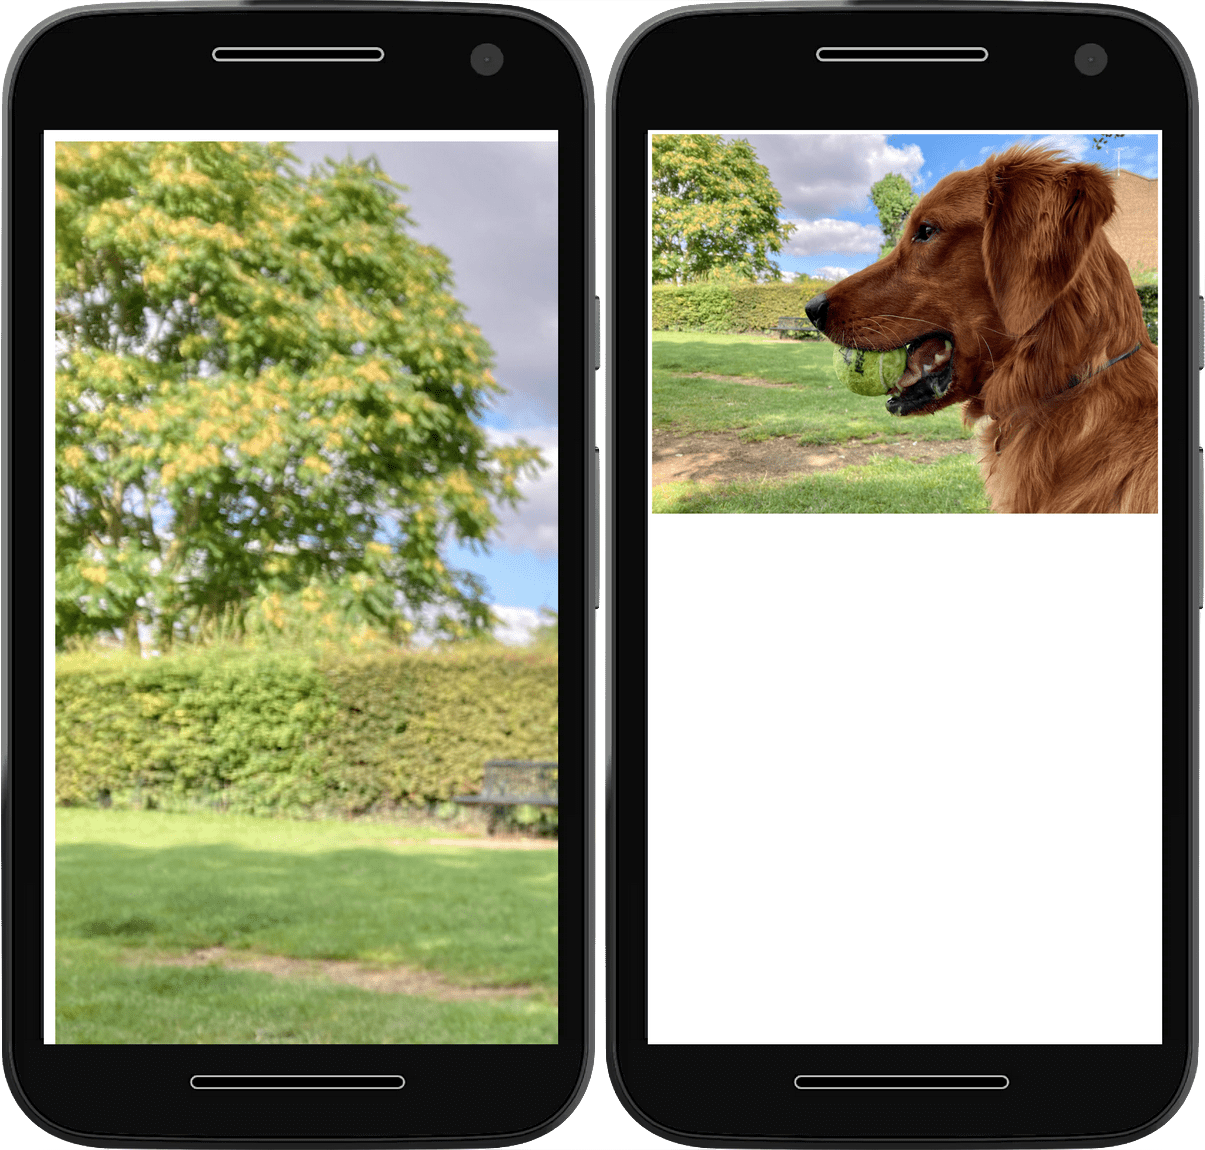
\includegraphics[width=0.68\linewidth]{online/webdev-responsive-image-layout.png}
\caption{图片超出视口与适应视口的直观对比}%
\label{fig:loading-online}
\end{figure}

图\ref{fig:loading-online}说明了图片首先应在页面中完整、合理地显示。%
但显示合适与下载合适是两个问题，后者还需要资源规格配合。

响应式图片通过 srcset 提供多个候选资源，通过 sizes 描述显示条件，%
让浏览器结合布局与像素密度选择图片\cite{responsive-images}。优点是减少不必要的大图传输，%
代价是需要生成和维护多尺寸文件。当前正文图片有懒加载和异步解码，但安全规则只允许受控地址，%
不能直接让文章作者写入任意 srcset。合理的扩展应由媒体服务提供可信候选，而不是绕过白名单。

\begin{table}[!htb]
\centering
\smalltable
\caption{容易被混为一谈的加载优化}
\begin{tabularx}{\linewidth}{>{\raggedright\arraybackslash}p{2.45cm}YY}
\toprule
技术 & 主要减少什么 & 使用时的注意点\\
\midrule
路由懒加载 & 尚未访问页面的初始代码 & 首次导航存在等待，应提供状态反馈\\
\tabledivider
图片懒加载 & 暂时不需要显示的图片请求 & 真正的首屏关键图片不宜延迟发现\\
\tabledivider
分页 & 单次读取和显示的数据数量 & 需要维护页码、筛选条件与返回行为\\
\tabledivider
虚拟列表 & 长列表同时存在的 DOM 节点 & 高度、焦点与滚动恢复更复杂，不会自动减少全部数据请求\\
\tabledivider
流式内容交付 & 等待完整结果后才开始显示的时间 & 需处理分段错误、加载边界和渐进呈现\\
\bottomrule
\end{tabularx}
\end{table}

由此我认识到，“越晚加载越快”也不准确。首屏最重要的图片应尽早被发现，非首屏图片再按需获取；%
用户主动打开编辑页后，必需的编辑能力也不应被无意义地拖延。性能优化更像安排工作顺序：%
先完成影响当前任务的部分，再处理其余内容，而不是对所有资源使用同一个开关。

\section{从输入文字到内容编辑}
\subsection{为什么需要研究编辑器}
公开文章只需要读，而后台必须能写。WEMOVE 的编辑任务不仅包括输入段落，还包括左右图文、通栏图片、%
替代文字、图注、段落顺序和预览。最初看上去，这些只是给输入框增加几个按钮；%
进一步阅读代码后，我发现编辑器还必须维护光标、选区、粘贴内容和保存格式，复杂度远高于一个普通文本框。

textarea 保存纯文本，结构简单、行为容易预测；contenteditable 让浏览器中的元素变为可编辑区域，%
能够处理富文本，却把生成的 DOM 与应用数据同步问题交给开发者\cite{mdn-contenteditable}。%
当前 ArticleTextField 使用 contenteditable，格式按钮调用 execCommand，粘贴时借助 Selection 与 Range
插入经过清洗的内容\cite{local-code}。我因此理解到，原生编辑能力可以降低起步成本，%
但不是一套完整的内容管理方案。

MDN 已将 execCommand 标记为弃用；其部分编辑操作仍与浏览器撤销历史有关，不能简单用几次 DOM
修改就替换所有行为\cite{mdn-execcommand}。这提醒我，%
技术“目前还能运行”和“适合作为长期扩展基础”是两回事。对本项目，需要关注中文输入法、粘贴、撤销重做、%
选区恢复和不同浏览器行为，而不是只验证点击加粗按钮后出现了粗体。

\subsection{项目中的图文区块：用约束换取稳定}
当前项目把正文组织成文字块、左右图文块和通栏图片，并分别维护图注与替代文字。%
管理员通过按钮选择布局、移动区块和插入图片，不需要直接手写任意 HTML。%
这类似一组规定了连接方式的积木：组合仍有自由，但每块内容的含义更明确。

\begin{figure}[H]
\centering
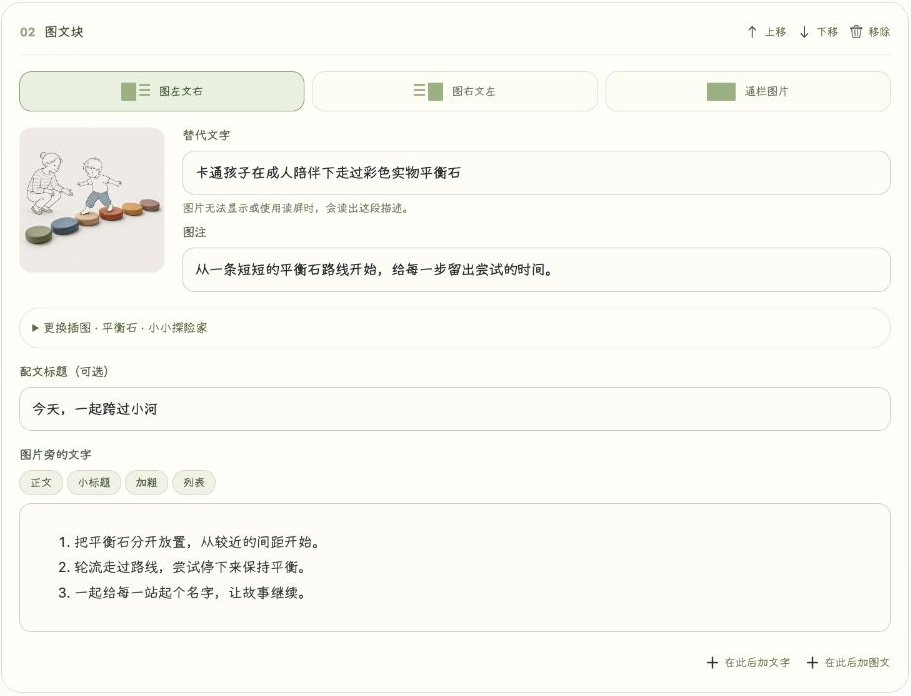
\includegraphics[width=0.94\linewidth]{文章区块编辑器.png}
\caption{本项目图文编辑器的开发预览界面}%
\label{fig:editor-project}
\end{figure}

项目保存的是受控 HTML，编辑时解析成区块，展示时再映射成允许的节点。这样可以兼容已有段落与列表，%
但也要求“打开—编辑—保存—再打开”后内容语义保持稳定。若用户移除一张正文图，%
它就不应又从独立图库中出现；若选择右图左文，手机端也要保持合理的阅读顺序。%
编辑器的质量不仅是输入时顺手，还包括数据离开编辑器之后能否正确使用。

\subsection{结构化编辑器的发展：文档模型成为核心}
为理解更复杂的编辑需求，我进一步调研 ProseMirror 和 Tiptap。ProseMirror 将文档结构、%
编辑状态和事务等概念明确组织起来；schema 规定哪些节点、标记及嵌套关系合法，%
事务描述一次编辑如何改变状态\cite{prosemirror-guide}。可以把 schema 理解为语法规则，%
把事务理解为有记录的修改指令。编辑不再只是任意修改网页节点，而是通过模型管理文档变化。

Tiptap 基于 ProseMirror 提供扩展式编辑器能力，并支持与 Vue 等框架集成\cite{tiptap-intro}。%
现代编辑器往往仍利用 contenteditable 接收浏览器输入，进步在于其上建立更明确的文档模型，%
并非抛弃浏览器的输入基础。这种路线的优势是更容易组织自定义节点、命令、选区和编辑扩展；%
代价是需要理解新的文档模型及插件生命周期，并处理现有 HTML 与新模型之间的迁移。%
无头编辑器没有强制的完整界面，给了我保持网站风格的空间，也意味着工具栏、%
交互反馈和可访问性仍需自己设计。

\begin{figure}[H]
\centering
\begin{tikzpicture}[font=\fontsize{11}{15}\selectfont,
 box/.style={draw=wmaccent,fill=wmnavy!5,rounded corners=2pt,%
   text width=4.8cm,minimum height=1.1cm,align=center},
 arr/.style={-{Stealth[length=2mm]},draw=wmaccent,line width=0.8pt}]
\node[box] (event) at (0,0) {\textbf{DOM event}\\%
  用户输入与浏览器事件};
\node[box] (transaction) at (7,0) {\textbf{Transaction}\\%
  把编辑表达为一次状态变换};
\node[box] (state) at (7,-2.1) {\textbf{new EditorState}\\%
  形成新的文档与选区状态};
\node[box] (view) at (0,-2.1) {\textbf{EditorView}\\%
  将状态呈现为可编辑界面};
\draw[arr] (event)--(transaction);%
\draw[arr] (transaction)--(state);
\draw[arr] (state)--(view);%
\draw[arr] (view)--(event);
\end{tikzpicture}

\caption{结构化编辑器的状态与文档处理机制}%
\label{fig:editor-online}
\end{figure}

\begin{table}[!htb]
\centering
\smalltable
\caption{内容编辑方案的优缺点}
\begin{tabularx}{\linewidth}{>{\raggedright\arraybackslash}p{2.7cm}YY}
\toprule
方案 & 主要优点 & 主要限制\\
\midrule
纯文本 & 输入直观、保存简单 & 缺少标题、图片等丰富结构\\
\tabledivider
Markdown & 用标记表达结构，便于保存和版本比较 & 标记语法有学习成本，复杂图文布局需扩展约定\\
\tabledivider
原生 contenteditable &
    可以快速建立所见即所得输入区 &
    选区、撤销、输入法、粘贴和浏览器差异需自行处理\\
\tabledivider
自制受控区块 & 贴合项目内容，布局和数据规则清楚 & 每增加一种复杂编辑能力都要维护对应交互和往返逻辑\\
\tabledivider
ProseMirror / Tiptap &
    文档模型与扩展机制较完整，适合持续扩展 &
    学习成本、内容迁移和插件维护工作更高\\
\bottomrule
\end{tabularx}
\end{table}

\subsection{多人编辑和安全：编辑能力的两条边界}
保存版本检查与实时协同编辑是不同能力。本项目提交 expectedVersion，%
当服务器发现用户依据的是旧版本时拒绝覆盖；它解决的是“不要悄悄盖掉别人已保存的修改”，%
并没有合并两人同时输入的文字。Yjs 使用 CRDT（无冲突复制数据类型）处理并发修改的同步与合并，%
可以与编辑器结合\cite{yjs-intro}。CRDT 按预设规则合并副本的修改，使收到同一组更新的副本最终一致，%
但不保证修改在内容含义上互不矛盾。这也会增加协作服务、持久化、身份、断线恢复和模型兼容的工作，%
当前课程需求没有要求我引入完整协作系统。

编辑器越自由，保存与展示的边界越要清楚。格式化输入本身不保证内容安全，富文本中的脚本、%
事件属性和危险地址需要过滤。当前服务端清洗 HTML，前端 ContentBody
再以白名单节点渲染\cite{local-code,owasp-xss}。因此，即使以后更换 Tiptap，%
也不能顺便删除现有的服务端规则。对我而言，编辑器的发展方向是更有组织地表达内容和修改过程，%
而不是无限制地接受任何网页片段。

\section{让展示适应不同使用条件}
\subsection{布局适配不仅是缩小页面}
在宽屏文章中，图片与文字可以并列；到了手机上，若仍强行保留两列，正文就可能窄得难以阅读。%
因此，本项目通过 Grid、Flexbox 和媒体查询调整布局，文章图文在窄屏转为单列。%
这里的目标是重新安排阅读空间，而不是把整个桌面页面等比例缩小。

进一步调研时，我了解到容器查询：媒体查询常依据视口等条件判断，%
容器查询可以依据组件所在容器的尺寸改变样式\cite{mdn-container}。同一个图文块可能处在宽文章区，%
也可能处在后台狭窄的预览栏，此时容器宽度比“是不是手机”更有意义。其优点是有助于组件复用，%
代价是需要设计查询容器和回退布局。当前项目主要使用媒体查询，容器查询属于我后续研究的方向。

\begin{figure}[H]
\centering
\begin{tikzpicture}[
  font=\fontsize{10.5}{14}\selectfont,
  line width=0.6pt,draw=wmnavy!65,
  labeltext/.style={text=wmnavy,align=left},
  wire/.style={draw=wmnavy!40,line width=0.5pt}
]
\node[anchor=west,font=\fontsize{11}{14}\selectfont\bfseries,text=wmnavy]
  at (0,0.55) {宽容器：图文两列};
\node[anchor=west,font=\fontsize{11}{14}\selectfont\bfseries,text=wmnavy]
  at (10.1,0.55) {窄容器：顺序堆叠};
\draw[rounded corners=3pt] (0,0) rectangle (9.1,-5.0);
\draw[rounded corners=3pt] (10.1,0) rectangle (14.6,-6.25);
\draw[wire] (0,-0.45) -- (9.1,-0.45);
\draw[wire] (10.1,-0.45) -- (14.6,-0.45);
\fill[wmnavy!25] (0.24,-0.23) circle (0.035);
\fill[wmnavy!25] (0.40,-0.23) circle (0.035);
\fill[wmnavy!25] (0.56,-0.23) circle (0.035);
\fill[wmnavy!25] (10.34,-0.23) circle (0.035);
\fill[wmnavy!25] (10.50,-0.23) circle (0.035);
\fill[wmnavy!25] (10.66,-0.23) circle (0.035);
\node[anchor=north west,labeltext,font=\fontsize{11}{14}\selectfont\bfseries]
  at (0.4,-0.85) {01\quad 内容标题};
\node[anchor=north west,labeltext,text width=3.65cm]
  at (0.4,-1.65) {02\quad 正文段落\\以语义顺序组织内容，\\保持段落层级清楚。};
\draw[wire] (0.5,-3.55) -- (3.85,-3.55);
\draw[wire] (0.5,-3.85) -- (3.85,-3.85);
\draw[wire] (0.5,-4.15) -- (3.10,-4.15);
\draw[fill=wmnavy!5,draw=wmnavy!50] (4.75,-1.0) rectangle (8.6,-3.30);
\draw[wire] (4.75,-1.0) -- (8.6,-3.30);
\draw[wire] (8.6,-1.0) -- (4.75,-3.30);
\node[fill=white,text=wmnavy,inner sep=4pt] at (6.675,-2.15) {03\quad 内容图片};
\node[anchor=north west,labeltext,text width=3.7cm] at (4.75,-3.57)
  {04\quad 图注说明};
\node[anchor=north west,labeltext,font=\fontsize{11}{14}\selectfont\bfseries]
  at (10.45,-0.78) {01\quad 内容标题};
\node[anchor=north west,labeltext,text width=3.6cm]
  at (10.45,-1.48) {02\quad 正文段落\\以语义顺序组织内容，\\保持段落层级清楚。};
\draw[fill=wmnavy!5,draw=wmnavy!50] (10.5,-3.42) rectangle (14.2,-5.24);
\draw[wire] (10.5,-3.42) -- (14.2,-5.24);
\draw[wire] (14.2,-3.42) -- (10.5,-5.24);
\node[fill=white,text=wmnavy,inner sep=4pt] at (12.35,-4.33) {03\quad 内容图片};
\node[anchor=north west,labeltext,text width=3.55cm] at (10.45,-5.48)
  {04\quad 图注说明};
\node[anchor=north west,labeltext,text width=8.65cm] at (0,-5.35)
  {同一内容结构：标题 → 正文 → 图片 → 图注。\\视觉列数变化时，阅读与键盘访问顺序保持合理。};
\node[anchor=north west,labeltext,text width=14.4cm] at (0,-6.65)
  {布局响应可用宽度，并尊重“减少动态效果”偏好。图片的 alt 属性提供替代文本，图注补充可见语境；%
    装饰性图片可使用空替代文本。};
\end{tikzpicture}

\caption{图文组件从并列到单列，内容语义保持一致}%
\label{fig:responsive}
\end{figure}

\subsection{动效与可访问性需要一起考虑}
页面入场效果使用浏览器 Web Animations API，并通过 IntersectionObserver
判断元素进入视口的情况\cite{local-code,mdn-waapi}。%
它比为每一个元素单独处理滚动事件更容易组织观察逻辑，但观察回调并不意味着任务没有计算成本，%
动画也不应遮挡交互。项目在减少动画偏好、焦点进入以及能力不足时提供更直接的内容显示方式。

我也逐渐理解，替代文字 alt 与图注并不相同。alt 传达看不到图片时需要知道的信息，%
图注解释画面与正文的联系；一幅装饰图与一张玩法说明图，不应机械使用同样的描述。%
类似地，菜单不能只有鼠标悬停才能使用，状态不能只靠颜色表达，键盘焦点也需要清楚可见。%
WCAG 2.2 提供相应的可访问性要求，但有几个合规属性并不意味着整站已通过审计\cite{wcag22}。

\subsection{用指标衡量体验感}
调研性能时，我接触到 LCP、INP 和 CLS：它们分别关注主要内容显示、交互响应和布局稳定性，%
良好阈值为不超过 2.5 秒、200 毫秒和 0.1，通常按移动端与桌面端分别观察访问的第 75
百分位\cite{web-vitals}。这些指标帮助我把“页面有点慢”拆成更具体的问题，%
但本文没有把行业阈值当作项目实测结果。

例如，图片迟到可能影响主要内容显示；编辑时同步处理很大的正文可能延迟输入反馈；%
没有预留图片空间可能让按钮突然移动。只减小打包文件不能同时解决这些问题，%
单次本地评分也不能代表所有用户。对这个项目，更合理的下一步是固定文章、设备和网络条件，%
分别比较资源请求、关键交互与布局变化，再决定优化重点。

\section{我的学习认识与总结}
\subsection{从记住工具名称到理解技术边界}
回顾这次任务，我的认识主要发生在三个方面。首先，前端技术之间有层次：HTML、CSS 和 JavaScript
是基础，Vue 帮助组织界面，TypeScript 与 Vite 改善工程过程，Three.js 和编辑器则服务于具体场景。%
它们不是越多越好，而是需要各自承担清楚的职责。

其次，相似的页面表现可能来自不同原理。卡片倾斜并不一定需要实体模型，%
懒加载代码并不等于图片或数据也已优化，能输入富文本也不代表已经拥有结构化文档或协同编辑。%
遇到需求时先确定要解决什么问题，再选择恰当层次的技术，比直接套用听起来先进的方案更有效。

最后，展示效果与稳定性需要一起考虑。三维效果要尊重性能和减少动画偏好；内容加载要处理失败与旧响应；%
编辑能力要保护文档结构和已有修改；图片和下载还受到安全与权限边界约束。%
对初学者来说，这些约束起初可能显得繁琐，实际却使前端从一次演示变成可以继续维护的应用。

\subsection{结合本项目的后续学习方向}
我的后续学习会继续沿着已有任务展开。三维方面，先深入理解坐标、透视和帧时间，%
再在确有模型展示需求时研究 glTF、WebGL 或 WebGPU；内容加载方面，先完善资源规格和测量，%
再评估公开文章的预渲染；编辑方面，优先研究输入法、撤销与文档往返，再判断是否迁移到结构化编辑器。%
这样的学习顺序能够把新知识与已有问题对应起来。

我也需要学习如何验证自己的判断。类型检查可以发现一类代码问题，组件测试可以检查状态变化，%
真实浏览器才能更直接地观察布局、焦点和输入体验。项目既有验证记录与本次技术调研承担不同作用；%
我没有把阅读官方示例写成实际部署，也没有把预览截图写成真实业务已经全部验收。%
对技术优缺点的认识，应在后续实践中继续被检验。

这份报告从前端入门出发，以 WEMOVE 的具体任务连接了三维展示、内容加载和内容编辑的现状。%
对我最有价值的收获，是能够解释一项技术为什么适合某个任务、又在哪些地方需要付出代价。%
前端的发展提供了更丰富的工具，而学习的目标是让这些工具帮助用户更顺畅地阅读、操作和维护内容。

\clearpage
\markboth{参考文献}{}
\begin{thebibliography}{99}
\addcontentsline{toc}{section}{参考文献}
\small\setlength{\itemsep}{0.55em}
\bibitem{mdn-basics}
MDN contributors. The web standards model[EB/OL]. [2026-09-08].
\url{https://developer.mozilla.org/en-US/docs/Learn_web_development/Getting_started/Web_standards/The_web_standards_model}.
\bibitem{vue-intro}
Vue.js. Introduction[EB/OL]. [2026-09-08].
\url{https://vuejs.org/guide/introduction}.
\bibitem{react-ui}
React. Describing the UI[EB/OL]. [2026-09-08].
\url{https://react.dev/learn/describing-the-ui}.
\bibitem{svelte-overview}
Svelte. Overview[EB/OL]. [2026-09-08].
\url{https://svelte.dev/docs/svelte/overview}.
\bibitem{ts-basics}
Microsoft. TypeScript Handbook: The Basics[EB/OL]. [2026-09-08].
\url{https://www.typescriptlang.org/docs/handbook/2/basic-types.html}.
\bibitem{vite-why}
Vite. Why Vite[EB/OL]. [2026-09-08].
\url{https://vite.dev/guide/why.html}.
\bibitem{local-team}
WEMOVE 项目组. WEMOVE 团队分工与协作规范：成员 E 职责[Z]. 本地仓库资料，核查日期：2026-09-08.
\path{project-implementation/project-requirements/WEMOVE团队分工与协作规范.md}.
\bibitem{local-code}
WEMOVE 项目组. 当前前端及后端内容源码：版本、路由、正文、媒体与动效[Z]. 本地仓库资料，核查日期：%
2026-09-08.
\path{project-implementation/apps/}.
\bibitem{element-dialog}
Element Plus. Dialog[EB/OL]. [2026-09-08].
\url{https://element-plus.org/en-US/component/dialog.html}.
\bibitem{three-css3d}
Three.js authors. CSS3DRenderer[EB/OL]. [2026-09-08].
\url{https://threejs.org/docs/pages/CSS3DRenderer.html}.
\bibitem{three-fundamentals}
Three.js authors. Fundamentals[EB/OL]. [2026-09-08].
\url{https://threejs.org/manual/en/fundamentals.html}.
\bibitem{mdn-webgpu}
MDN contributors. WebGPU API[EB/OL]. [2026-09-08].
\url{https://developer.mozilla.org/en-US/docs/Web/API/WebGPU_API}.
\bibitem{three-webgpu}
Three.js authors. WebGPURenderer[EB/OL]. [2026-09-08].
\url{https://threejs.org/manual/en/webgpurenderer.html}.
\bibitem{model-viewer}
model-viewer contributors. model-viewer[EB/OL]. [2026-09-08].
\url{https://modelviewer.dev/}.
\bibitem{router-lazy}
Vue Router. Lazy Loading Routes[EB/OL]. [2026-09-08].
\url{https://router.vuejs.org/guide/advanced/lazy-loading.html}.
\bibitem{vue-ssr}
Vue.js. Server-Side Rendering (SSR)[EB/OL]. [2026-09-08].
\url{https://vuejs.org/guide/scaling-up/ssr.html}.
\bibitem{nuxt-rendering}
Nuxt. Rendering Modes[EB/OL]. [2026-09-08].
\url{https://nuxt.com/docs/4.x/guide/concepts/rendering}.
\bibitem{astro-islands}
Astro. Islands architecture[EB/OL]. [2026-09-08].
\url{https://docs.astro.build/en/concepts/islands/}.
\bibitem{webdev-layout}
Google web.dev. Responsive images: Learn Design[EB/OL]. [2026-09-08].
\url{https://web.dev/learn/design/responsive-images}.
\bibitem{responsive-images}
Google web.dev. Responsive images: Learn Images[EB/OL]. [2026-09-08].
\url{https://web.dev/learn/images/responsive-images}.
\bibitem{vue-performance}
Vue.js. Performance[EB/OL]. [2026-09-08].
\url{https://vuejs.org/guide/best-practices/performance.html}.
\bibitem{web-lcp}
Google / web.dev. Optimize Largest Contentful Paint[EB/OL]. [2026-09-08].
\url{https://web.dev/articles/optimize-lcp}.
\bibitem{mdn-streams}
MDN contributors. Using readable streams[EB/OL]. [2026-09-08].
\url{https://developer.mozilla.org/en-US/docs/Web/API/Streams_API/Using_readable_streams}.
\bibitem{mdn-contenteditable}
MDN contributors. contenteditable global attribute[EB/OL]. [2026-09-08].
\url{https://developer.mozilla.org/en-US/docs/Web/HTML/Reference/Global_attributes/contenteditable}.
\bibitem{mdn-execcommand}
MDN contributors. Document: execCommand() method[EB/OL]. [2026-09-08].
\url{https://developer.mozilla.org/en-US/docs/Web/API/Document/execCommand}.
\bibitem{prosemirror-guide}
Marijn Haverbeke et al.. ProseMirror Guide[EB/OL]. [2026-09-08].
\url{https://prosemirror.net/docs/guide/}.
\bibitem{tiptap-intro}
Tiptap. Core concepts: Introduction[EB/OL]. [2026-09-08].
\url{https://tiptap.dev/docs/editor/core-concepts/introduction}.
\bibitem{yjs-intro}
Yjs contributors. Introduction[EB/OL]. [2026-09-08].
\url{https://docs.yjs.dev/}.
\bibitem{owasp-xss}
OWASP Foundation. Cross Site Scripting Prevention Cheat Sheet[EB/OL]. [2026-09-08].
\url{https://cheatsheetseries.owasp.org/cheatsheets/Cross_Site_Scripting_Prevention_Cheat_Sheet.html}.
\bibitem{mdn-container}
MDN Web Docs. CSS container queries[EB/OL]. [2026-09-08].
\url{https://developer.mozilla.org/en-US/docs/Web/CSS/Guides/Containment/Container_queries}.
\bibitem{mdn-waapi}
MDN contributors. Web Animations API[EB/OL]. [2026-09-08].
\url{https://developer.mozilla.org/en-US/docs/Web/API/Web_Animations_API}.
\bibitem{wcag22}
W3C. Web Content Accessibility Guidelines (WCAG) 2.2[EB/OL]. [2026-09-08].
\url{https://www.w3.org/TR/WCAG22/}.
\bibitem{web-vitals}
Google / web.dev. Web Vitals[EB/OL]. [2026-09-08].
\url{https://web.dev/articles/vitals}.
\end{thebibliography}

\end{document}
